\documentclass{standalone}
\usepackage{tikz} 
\usetikzlibrary{graphs} 
\usetikzlibrary{positioning} 
\usetikzlibrary{arrows.meta}
\begin{document}

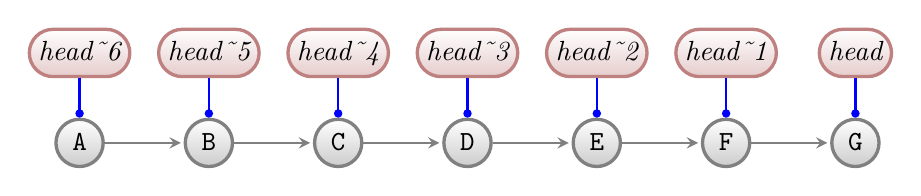
\begin{tikzpicture}[
nonterminal/.style={
	% The shape:
	rectangle,
	% The size:
	minimum size=6mm,
	% The border:
	very thick,
	draw=red!50!black!50, % 50% red and 50% black,
	% and that mixed with 50% white
	% The filling:
	top color=white, % a shading that is white at the top...
	bottom color=red!50!black!20, % and something else at the bottom
	% Font
	font=\itshape},
every node/.style={
	% The shape:
	rectangle,minimum size=6mm,rounded corners=3mm,
	% The rest
	very thick,draw=black!50,
	top color=white,bottom color=black!20,
	font=\ttfamily},
text height=1.5ex,text depth=.25ex,
>=stealth, thick, black!50, text=black,
every new ->/.style={shorten >=1pt},
graphs/every graph/.style={edges=rounded corners},
]

\graph [grow right sep = 10mm] { A -> B -> C -> D -> E -> F -> G
};

\node (head) [node distance=5mm, nonterminal,above =of G] {head};
\draw[-{Circle[length=3pt]},blue] (head) -- (G);
\node (head_1) [node distance=5mm, nonterminal,above =of F] {head\textasciitilde1};
\draw[-{Circle[length=3pt]},blue] (head_1) -- (F);
\node (head_2) [node distance=5mm, nonterminal,above =of E] {head\char`~2};
\draw[-{Circle[length=3pt]},blue] (head_2) -- (E);
\node (head_3) [node distance=5mm, nonterminal,above =of D] {head\char`~3};
\draw[-{Circle[length=3pt]},blue] (head_3) -- (D);
\node (head_4) [node distance=5mm, nonterminal,above =of C] {head\char`~4};
\draw[-{Circle[length=3pt]},blue] (head_4) -- (C);
\node (head_5) [node distance=5mm, nonterminal,above =of B] {head\char`~5};
\draw[-{Circle[length=3pt]},blue] (head_5) -- (B);
\node (head_6) [node distance=5mm, nonterminal,above =of A] {head\char`~6};
\draw[-{Circle[length=3pt]},blue] (head_6) -- (A);
\end{tikzpicture}

\end{document}
